% !TEX root =../thesis-letomes.tex

\chapter{Physical Modelling}
We will broadly 

\section{CM-Centered Restricted 3-Body System (C-R3B), Earth-Moon}
The center-of-mass-centered 3-body system (C-R3B) with the Earth and Moon was explored in \cite{Saxe2015}; refer to this for detailed derivations of C-R3B. We will present the final nondimensionalized equations of motion, and numerical integration algorithms for reference. The model is set up as in \cref{fig:r3b}.

\begin{figure}[ht!]
    \centering
    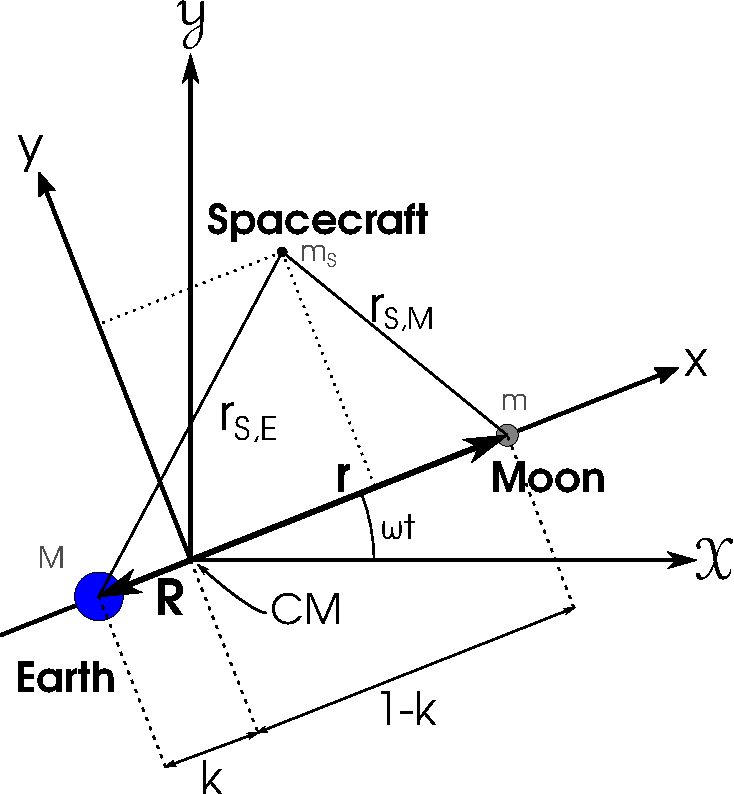
\includegraphics[scale=0.75]{fig/r3b.pdf}
    \caption{Restricted three-body problem. Two coordinate systems both with center of mass as origin: $(\mathscr{X},\mathscr{Y})$ is a stationary inertial frame, $(x,y)$ is a co-rotating non-inertial frame that rotates with the moon at angular frequency $\omega$. $M =$ mass of Earth, $m =$ mass of Moon, $\vec{R} =$ vector from CM to earth, $\vec{r} =$ vector from CM to Moon, $m_s =$ mass of spacecraft, $r_{S,E} =$ distance from spacecraft to Earth, $r_{S,M} =$ distance from spacecraft to Moon. In the dimensionless variables we introduce later, unit distance is $R+r$, which makes the dimensionless constant $k = \text{the CM-Earth distance} = \dfrac{R}{R+r} = $ and $1-k = \text{the CM-Moon distance} = \dfrac{r}{R+r}$ (Image: \cite{Saxe2015}).}
    \label{fig:r3b}
\end{figure}

\subsection{C-R3B Equations of Motion}

\begin{empheq}[box=\widefbox]{align}
\label{eq:Xdot}
\dot{X} = P_x + Y
\end{empheq}

\begin{empheq}[box=\widefbox]{align}
\label{eq:Ydot}
\dot{Y} = P_Y - X
\end{empheq}

\begin{empheq}[box=\widefbox]{align}
\label{eq:Pdot_X}
\dot{P}_X = P_Y - \dfrac{(1-k)(X+k)}{((X+k)^2+Y^2)^{3/2}} - \dfrac{k(X-1+k))}{((X-1+k))^2+Y^2)^{3/2}}
\end{empheq}

\begin{empheq}[box=\widefbox]{align}
\label{eq:Pdot_Y}
\dot{P}_Y = -P_X - \dfrac{(1-k)Y}{((X+k)^2+Y^2)^{3/2}} - \dfrac{k Y}{((X-1+k))^2+Y^2)^{3/2}}
\end{empheq}
where \(T\), \(X\), \(Y\), \(P_x\) and \(P_y\) are our dimensionless variables for time, positions, generalized impulse, and \(k=\dfrac{M_{\Moon}}{M_{\Earth} + M_{\Moon}}\), that is the ratio of Moon's mass to the total Moon and Earth mass.

\subsection{C-R3B Numerical Algorithms}
\subsubsection{C-R3B Symplectic Euler}
Based on \cref{eq:Xdot,eq:Ydot,eq:Pdot_X,eq:Pdot_Y}, a symplectic Euler algorithm was found (For detailed derivation, see \cite{Saxe2015}):

\begin{align}
    X_1 &= \dfrac{X_0 + h (h P_{Y,0} + P_{X,0} + Y_0)}{1+h^2}, \\[0.4cm]
    Y_1 &= Y_0 + h (P_{Y,0} - X_1), \label{eq:symplectic-euler-Y_1}
\end{align}
\begin{align}
    \begin{aligned}
        P_{X,1} &= P_{X,0} \\
        &+ h \left(P_{Y,0} - \dfrac{(1-k)(k+X_1)}{((k+X_1)^2+Y_1^2)^{3/2}} + \dfrac{k(X_1-1+k)}{((X_1-1+k)^2+Y_1^2)^{3/2}}\right), \label{eq:symplectic-euler-PX_1}
    \end{aligned} \\[0.4cm]
    \begin{aligned}
        P_{Y,1} &= P_{Y,0} \\
        &+ h \left(-P_{X,0} - \dfrac{(1-k)Y_1}{((k+X_1)^2+Y_1^2)^{3/2}} - \dfrac{k Y_1}{((X_1-1+k)^2+Y_1^2)^{3/2}}\right), \label{eq:symplectic-euler-PY_1}
    \end{aligned}
\end{align}
where \(h\) is the step size, index \(0\) designates previous time step ($i$) and index \(1\) designates new time step ($i+1$). The algorithm is run in the same order as listed above.

\subsubsection{C-R3B Symplectic Störmer-Verlet}
Based on \cref{eq:Xdot,eq:Ydot,eq:Pdot_X,eq:Pdot_Y}, a symplectic Störmer-Verlet algorithm was also found (For detailed derivation, see \cite{Saxe2015}):

\begin{align}
    X_{1/2} &= \frac{h^2 P_{Y,0} + 2 h \dot{P}_{x,0} + 4 X_0}{4 + h^2} \label{eq:verlet-x_1/2} \\
    Y_{1/2} &= Y_0 + \dfrac{h}{2} (P_{Y,0} - X_{1/2}), \label{eq:verlet-y_1/2} \\
    P_{X,1} &= \frac{h^2 (2 \dot{P}_{Y,0} + P_{X,0}) + 4 h \dot{P}_{X,0} + 4 P_{X,0} }{4 + h^2} \label{eq:verlet-px_1} \\
    P_{Y,1} &= P_{Y,0} + \dfrac{h}{2} \left[-\dot{P}_Y(q_{1/2},p_0) -\dot{P}_Y(q_{1/2},p_1) \right], \label{eq:verlet-py_1} \\
    X_1 &= X_{1/2} + \dfrac{h}{2} (P_{X,1} + Y_{1/2}), \label{eq:verlet-x_1} \\
    Y_1 &= Y_{1/2} + \dfrac{h}{2} (P_{Y,1} - X_{1/2}), \label{eq:verlet-y_1}
\end{align}
where \(\dot{P}_X,\dot{P}_Y\) are \cref{eq:Pdot_X,eq:Pdot_Y}, \(h\) is the step size, index \(0\) designates previous time step ($i$) and \(1\) designates new time step ($i+1$). The algorithm is run in the same order as listed above.

\section{Heliocentric Restricted 4-Body System (H-R4B), Sun-Earth-Mars}
Simulating orbit from Earth to Mars requires a new model with at least four bodies: Sun, Earth, Mars and the Spacecraft. The coordinate system will be heliocentric and in spherical coordinates, and restricted meaning that the mass of the spacecraft is considered negligible compared to compared to the celestial masses, so we call this system the ``Heliocentric Restricted N-Body'' system, see \cref{fig:solar-system-model}. We will derive the equations of motion of the spacecraft by using Hamilton's equations, which naturally gives us a set of coupled first-order differential equations, and a set of conserved quantities as ``generalized momenta''.

\begin{figure}[ht]
    \centering
    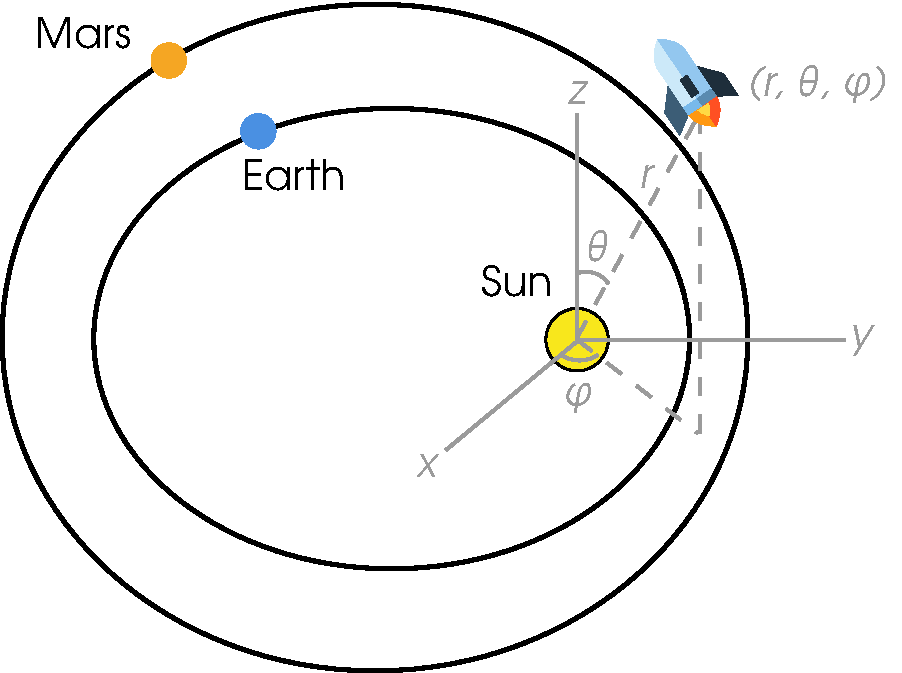
\includegraphics[width=0.80\linewidth]{fig/solar-system-model}
    \caption{ H-R4B model of spacecraft motion.The sun is assumed stationary at the origin of a spherical coordinate system, and the focus of two elliptical orbits of Earth and Mars. (Assets source: \cite{WikiSpherical,flaticon})}
    \label{fig:solar-system-model}
\end{figure}

\subsection{Spherical Coordinate System}
We adopt the spherical coordinate system which customary in astrodynamics, as shown in \cref{fig:solar-system-model}.

The coordinate transform equations to and from the cartesian coordinate system are:

\begin{align}
    x &= r \sin{\theta}\cos{\phi}, \label{eq:x(q)} \\
    y &= r \sin{\theta}\sin{\phi}, \label{eq:y(q)}\\
    z &= r \cos{\theta}, \label{eq:z(q)}
\end{align}

and

\begin{align}
    r &= \sqrt{x^2 + y^2 + z^2}, \label{eq:r(x,y,z)}\\
    \theta &= \arccos{\frac{z}{r}}, \label{eq:theta(x,y,z)}\\
    % \arctan{\frac{y}{x}}, \qquad \theta  \in [0, 2\pi]
    \phi &= 
    \arctantwo{(y/x)} \\
    \label{eq:phi(x,y,z)}
\end{align}

where \(r \in [0, \infty]\), \(\theta \in [0, \pi]\) and \(\phi \in [0, 2\pi]\) and \(\arctan2\) denotes the two-argument version of \(\arctan\) function \footnote{\(\arctan{(a)} \in (-\frac{\pi}{2}, \frac{\pi}{2})\) just takes a slope as input and give an angle in quadrant 1 and 4 only, whereas \(\arctantwo{(y,x)} \in (-\pi, \pi]\) takes both \(x\) and \(y\) which also gives the correct quadrant 1–4.}\cite{WikiAtan2}.

For the calculation of kinetic in the next section we will need the position vector, unit vectors in spherical coordinates, and the Jacobians.

The position vector in spherical coordinates is
\begin{align}
    \vec{r}(r, \theta, \phi) &= x \xhat + y \yhat + z \zhat \\
    \Leftrightarrow \vec{r}(r, \theta, \phi) &= r \sin{\theta}\cos{\phi} \xhat + r \sin{\theta}\sin{\phi} \yhat + r \cos{\theta} \zhat. \label{eq:position-vec-spherical}
\end{align}

The various coordinate derivatives of the position vector is
\begin{align}
    \pd{\vec{r}}{r} &= \sin{\theta}\cos{\phi} \xhat + \sin{\theta}\sin{\phi} \yhat + \cos{\theta} \zhat \quad &\text{and} \quad &\left| \pd{\vec{r}}{r} \right| = 1 \label{eq:position-derived-r} \\
    \pd{\vec{r}}{\theta} &= r \cos{\theta}\cos{\phi} \xhat + r \cos{\theta}\sin{\phi} \yhat - r \sin{\theta} \zhat \quad &\text{and} \quad &\left| \pd{\vec{r}}{\theta} \right| = r \label{eq:position-derived-theta} \\
    \pd{\vec{r}}{\phi} &= -r\sin{\theta}\sin{\phi} \xhat + r\sin{\theta}\cos{\phi} \zhat \quad &\text{and} \quad &\left| \pd{\vec{r}}{\phi} \right| = r\sin{\theta} \label{eq:position-derived-phi}
\end{align}

So the unit vectors in spherical coordinates are
\begin{align}
    \rhat = \dfrac{\pd{\vec{r}}{r}}{\left| \pd{\vec{r}}{r} \right| } &= \sin{\theta}\cos{\phi} \xhat + \sin{\theta}\sin{\phi} \yhat + \cos{\theta} \zhat \label{eq:r-hat}\\
    \thetahat = \dfrac{\pd{\vec{r}}{\theta}}{\left| \pd{\vec{r}}{\theta} \right| } &= \cos{\theta}\cos{\phi} \xhat + \cos{\theta}\sin{\phi} \yhat - \sin{\theta} \zhat \label{eq:theta-hat}\\
    \phihat = \dfrac{\pd{\vec{r}}{\phi}}{\left| \pd{\vec{r}}{\phi} \right| } &= -\sin{\phi} \xhat + \cos{\phi} \zhat \label{eq:phi-hat}
\end{align}

\subsection{H-R4B Equations of Motion}
We will follow the 5-step process of arriving at Hamilton's equations outlined in \cref{apx:hamiltons}.

\subsubsection{Step 1: Lagrangian \(L\)}
The kinetic energy of the system is
\begin{align}
    T = \frac{1}{2} m_s v^2.
\end{align}

In general the total derivative of a vector is:

\begin{align}
    \vec{v} &= \od{\vec{r}}{t} = \sum\limits_{j} \pd{\vec{r}}{q_j} \od{q_j}{t}, \\
      &= \sum\limits_{j} \left|\pd{\vec{r}}{q_j}\right| \frac{\pd{\vec{r}}{q_j}}{\left|\pd{\vec{r}}{q_j}\right|} \od{q_j}{t}, \\
      &= \sum\limits_{j} \left|\pd{\vec{r}}{q_j}\right| \od{q_j}{t} \unitvector{q}_j, \\
      &= \sum\limits_{j} \left|\pd{\vec{r}}{q_j}\right| \dot{q_j} \unitvector{q}_j,
    \end{align}

where we have used that a unit vector for any coordinate system is \(\frac{\pd{\vec{r}}{q_j}}{\left|\pd{\vec{r}}{q_j}\right|} = \unitvector{q}_j\).
We can now use the derivatives of the position vector we found earlier in \cref{eq:position-derived-r,eq:position-derived-theta,eq:position-derived-phi}, to substitute for \(\left|\pd{\vec{r}}{q_j}\right|\). We don't have to substitute in \(\unitvector{q}_j\) since our unit vectors are orthogonal, so they will yield either 0 or 1 when we square \(v\). So for the spherical coordinates we get:

\begin{align}
    \vec{v} = \dot{r}\rhat + r\dot{\theta}\thetahat + r\sin{\theta}\,\dot{\phi}\phihat
\end{align}

so

\begin{align}
    v^2 = \dot{r}^2 + r^2\dot{\theta}^2 + r^2\sin^2{\theta}\,\dot{\phi}^2
\end{align}

so we get

\begin{align}
    T = \frac{1}{2} m_s (\dot{r}^2 + r^2\dot{\theta}^2 + r^2\sin^2{\theta}\,\dot{\phi}^2).
\end{align}

The gravitational potential is \cite{WikiGravPotential}

\begin{align}
    V = -G m_s \sum\limits_{k} \frac{M_k}{\left| \vec{r} - \vec{r_k} \right|},
\end{align}
where \(i\) denotes the celestial bodies acting on the spacecraft, i.e. in our system Sun, Earth and Mars.

So we finally get the Lagrangian

\begin{align}
    L &= T - V \\
    \Leftrightarrow L &= \frac{1}{2} m_s (\dot{r}^2 + r^2\dot{\theta}^2 + r^2\sin^2{\theta}\,\dot{\phi}^2) + G m_s \sum\limits_{k} \frac{M_k}{\left| \vec{r} - \vec{r_k} \right|}
\end{align}

\subsubsection{Step 2: Generalized Momenta \(p_j\)}
\begin{align}
    p_r &= \pd{L}{\dot{r}} = m_s \dot{r} \label{eq:pr} \\
    p_\theta &= \pd{L}{\dot{\theta}} = m_s r^2 \dot{\theta} \label{eq:ptheta} \\
    p_\phi &= \pd{L}{\dot{\phi}} = m_s r^2 \sin^2{\theta} \dot{\phi} \label{eq:pphi}
\end{align}

\subsubsection{Step 3: \(\dot{q} = \dot{q}_j(\vec{q}, \vec{p}, t)\)}
\begin{align}
    \dot{r} &= \frac{p_r}{m_s} \\
    \dot{\theta} &= \frac{p_\theta}{m_s r^2} \\
    \dot{\phi} &= \frac{p_\phi}{m_s r^2 \sin^2{\theta}}
\end{align}

We can now rewrite \(L\) to make it independent of \(\dot{q}\) by substituting the expressions above:

\begin{align}
    T &= \frac{1}{2} m_s (\dot{r}^2 + r^2\dot{\theta}^2 + r^2\sin^2{\theta}\,\dot{\phi}^2) \\
    &= \frac{1}{2} m_s \left(\frac{p_r^2}{m_s^2} + r^2\frac{p_\theta^2}{m_s^2 r^4} + r^2\sin^2{\theta}\frac{p_\phi^2}{m_s^2 r^4 \sin^4{\theta}} \right) \\
    &= \frac{p_r^2}{2 m_s} + \frac{p_\theta^2}{2 m_s r^2} + \frac{p_\phi^2}{2 m_s r^2 \sin^2{\theta}} \\
\end{align}

So using \(L = T - V\) we have

\begin{align}
    L = \frac{p_r^2}{2 m_s} + \frac{p_\theta^2}{2 m_s r^2} + \frac{p_\phi^2}{2 m_s r^2 \sin^2{\theta}} + G m_s \sum\limits_{k} \frac{M_k}{\left| \vec{r} - \vec{r_k} \right|}
\end{align}

\subsubsection{Step 4: Hamiltonian \(H\)}
\begin{align}
    H(\vec{q}, \vec{p}, t) &= \sum\limits_{j}p_j \dot{q_j} - L \\
    &= \sum\limits_{j}p_j \dot{q_j}(\vec{q}, \vec{p}, t) - L \\
    &= p_r \frac{p_r}{m_s} + p_\theta \frac{p_\theta}{m_s r^2} + p_\phi + \frac{p_\phi}{m_s r^2 \sin^2{\theta}} \notag \\
    &- \left( \frac{p_r^2}{2 m_s} + \frac{p_\theta^2}{2 m_s r^2} + \frac{p_\phi^2}{2 m_s r^2 \sin^2{\theta}} + G m_s \sum\limits_{k} \frac{M_k}{\left| \vec{r} - \vec{r_k} \right|} \right) \\
    \Leftrightarrow H &= \frac{p_r^2}{2 m_s} + \frac{p_\theta^2}{2 m_s r^2} + \frac{p_\phi^2}{2 m_s r^2 \sin^2{\theta}} - G m_s \sum\limits_{k} \frac{M_k}{\left| \vec{r} - \vec{r_k} \right|}
\end{align}

At this point we want to expand the expression \(\left| \vec{r} - \vec{r_k} \right|\) in anticipation of needing to differentiate \(H\) with respect to the coordinates. Using the equations for the \(x, y, z\) coordinates \cref{eq:x(q),eq:y(q),eq:z(q)} we get

\begin{align}
    d_k = \left|\vec{r} - \vec{r}_k \right| &= \sqrt{(x-x_k)^2 + (y-y_k)^2 + (z-z_k)^2}
\end{align}
and
\begin{align}
    (x-x_k)^2 &= (r\sin{\theta}\cos{\phi} - r\sin{\theta}\cos{\phi})^2 \notag \\
    &= \tikz[baseline]{
        \node[fill=orange!20,anchor=base]
        {\(r^2\sin^2{\theta}\cos^2{\phi}\)}
    } + \tikz[baseline]{
        \node[fill=red!20,anchor=base]
        {\(r_k^2\sin^2{\theta_k}\cos^2{\phi_k}\)}
    } - 2r r_k \sin{\theta}\sin{\theta_k}\cos{\phi}\cos{\phi_k} \label{eq:x-dist-squared} \\
    (y-y_k)^2 &= (r\sin{\theta}\sin{\phi} - r\sin{\theta}\sin{\phi})^2 \notag \\
    &= \tikz[baseline]{
        \node[fill=orange!20,anchor=base]
        {\(r^2\sin^2{\theta}\sin^2{\phi}\)}
    } + \tikz[baseline]{
        \node[fill=red!20,anchor=base]
        {\(r_k^2\sin^2{\theta_k}\sin^2{\phi_k}\)}
    } - 2r r_k \sin{\theta}\sin{\theta_k}\sin{\phi}\sin{\phi_k} \label{eq:y-dist-squared} \\
    (z-z_k)^2 &= (r\cos{\theta} - r\cos{\theta})^2 \notag \\
    &= \tikz[baseline]{
        \node[fill=orange!20,anchor=base]
        {\(r^2\cos^2{\theta}\)}
    } + \tikz[baseline]{
        \node[fill=red!20,anchor=base]
        {\(r_k^2\cos^2{\theta_k}\)}
    } - 2r r_k \cos{\theta}\cos{\theta_k}. \label{eq:z-dist-squared}
\end{align}
Now adding all three \cref{eq:x-dist-squared,eq:y-dist-squared,eq:z-dist-squared} the orange terms add to \(r^2\) and the red terms add to \(r_k^2\) and we get

\begin{align}
    d_k &= \sqrt{
        \tikz[baseline]{\node[fill=orange!20,anchor=base]{\(r^2\)}}
        + \tikz[baseline]{\node[fill=red!20,anchor=base]{\(r_k^2\)}}
        -2r r_k(\cos{\theta}\cos{\theta_k}+\sin{\theta}\sin{\theta_k}(
            \tikz[baseline]{\node[fill=blue!20,anchor=base]{
                \(\cos{\phi}\cos{\phi_k} + \sin{\phi}\sin{\phi_k}\)}}
        ))
    } \\
    &= \sqrt{r^2 + r_k^2 - 2 r r_k(\cos{\theta}\cos{\theta_k}+\sin{\theta}\sin{\theta_k}\cos{(\phi - \phi_k}))},
\end{align}
where the blue factor was simplified using the sum rule \cite{WeissteinTrig}: \\
\(\cos{\alpha}\cos{\beta} + \sin{\alpha}\sin{\beta} = cos{\alpha-\beta}\).

So we can finally express \(H\) as
\begin{equation}
    \begin{aligned}
        H &= \frac{p_r^2}{2 m_s} + \frac{p_\theta^2}{2 m_s r^2} + \frac{p_\phi^2}{2 m_s r^2 \sin^2{\theta}} \\
        &- G m_s \sum\limits_{k} \frac{M_k}{\sqrt{r^2 + r_k^2 - 2 r r_k \left[\cos{\theta}\cos{\theta_k}+\sin{\theta}\sin{\theta_k}\cos{(\phi - \phi_k})\right]}}
    \end{aligned}
\end{equation}

\subsubsection{Step 5: Hamilton's Equations}
\begin{align}
    \dot{r} = \pd{H}{p_r} &= \frac{p_r}{m_s} \label{eq:rdot} \\[0.3cm]
    \dot{\theta} = \pd{H}{p_\theta} &= \frac{p_\theta}{m_s r^2} \label{eq:thetadot} \\[0.3cm]
    \dot{\phi} = \pd{H}{p_\phi} &= \frac{p_\phi}{m_s r^2 \sin^2{\theta}} \label{eq:phidot}  \\[0.3cm]
    \begin{split}
        \dot{p}_r = -\pd{H}{r} &= \frac{p_\theta^2}{m_s r^3} + \frac{p_\phi^2}{m_s r^3 \sin^2{\theta} } \\
        &+ G m_s \sum\limits_{k} M_k \frac{-r + r_k \left(\cos{\theta}\cos{\theta_k} + \sin{\theta}\sin{\theta_k}\cos{(\phi - \phi_k)}\right)}{\left[r^2 + r_k^2 - 2 r r_k \left(\cos{\theta}\cos{\theta_k} + \sin{\theta}\sin{\theta_k}\cos{(\phi - \phi_k)} \right) \right]^{3/2}} \label{eq:prdot}
    \end{split} \\[0.3cm]
    \begin{split}
        \dot{p}_\theta = -\pd{H}{\theta} &= \frac{p_\phi^2}{m_s r^2 \sin^2{\theta} \tan{\theta}} \\
        &+ G m_s \sum\limits_{k} M_k \frac{r r_k \left[-\sin{\theta}\cos{\theta_k} + \cos{\theta}\sin{\theta_k}\cos{(\phi - \phi_k)} \right]}{\left[r^2 + r_k^2 - 2 r r_k \left(\cos{\theta}\cos{\theta_k} + \sin{\theta}\sin{\theta_k}\cos{(\phi - \phi_k)} \right) \right]^{3/2}} \label{eq:pthetadot}
    \end{split} \\[0.3cm]
    \begin{split}
        \dot{p}_\phi = -\pd{H}{\phi} &= G m_s \sum\limits_{k} M_k \frac{- r r_k \sin{\theta}\sin{\theta_k}\sin{(\phi - \phi_k)}}{\left[r^2 + r_k^2 - 2 r r_k \left(\cos{\theta}\cos{\theta_k} + \sin{\theta}\sin{\theta_k}\cos{(\phi - \phi_k)} \right) \right]^{3/2}} \label{eq:pphidot}
    \end{split}
\end{align}

Those are our equations of motion. However before we try to solve them, we will remove all units.

\subsection{H-R4B Equations Nondimensionalized}
We will now choose suitable characteristic units, which has a number of benefits:
\begin{itemize}
    \item The equations gets slightly simplified
    \item The order of the effects of different forces in the system becomes more apparent.
    \item Many of the calculations in numerical algorithms happens at an order of about 1. 
\end{itemize}

The characteristic units are chosen as:
\begin{align}
    \text{Unit length: } k_r &= a_{\Earth}\ {\color{gray} \approx \SI{1.50e8}{\km}}  \\[0.2cm]
    \text{Unit time: } k_t &= T_{\Earth} = \frac{2\pi}{\omega_\Earth} = 2\pi \sqrt{\frac{a_\Earth^3}{G M_\Sun}}\ {\color{gray} \approx \SI{3.16e7}{\s} \text{ (1 year)}} \\[0.2cm]
    \text{Unit speed: } k_v &= \frac{k_r}{k_t} = \frac{a_\Earth \omega_\Earth}{2\pi} = \frac{1}{2\pi} \sqrt{\frac{G M_\Sun}{a_\Earth}}\ {\color{gray} \approx \SI{4.74}{\km/\s}}
\end{align}
where \(a_\Earth\) is the semi-major axis of Earth's orbit in kilometers, see \cref{fig:earth-semi-major-axis}, \(T_\Earth\) is Earth's orbital period (i.e. 1 year) in seconds and the characteristic speed thus becomes Earth's average orbital speed with respect to the sun.

We don't need a characteristic mass \(m_s\) since the mass cancels out in the equations of motion for the quantity we care about, delta-v.

The unit for time is expressed in seconds because we found heuristically we needed time steps on the order of \(\SI{1}{\s}\) to maintain an error per step of about \num{10e-9}.

The unit for length is expressed in kilometers because it is customary to use \si{\km/\s} as unit of speed for celestial objects.

\begin{figure}[ht]
    \centering
    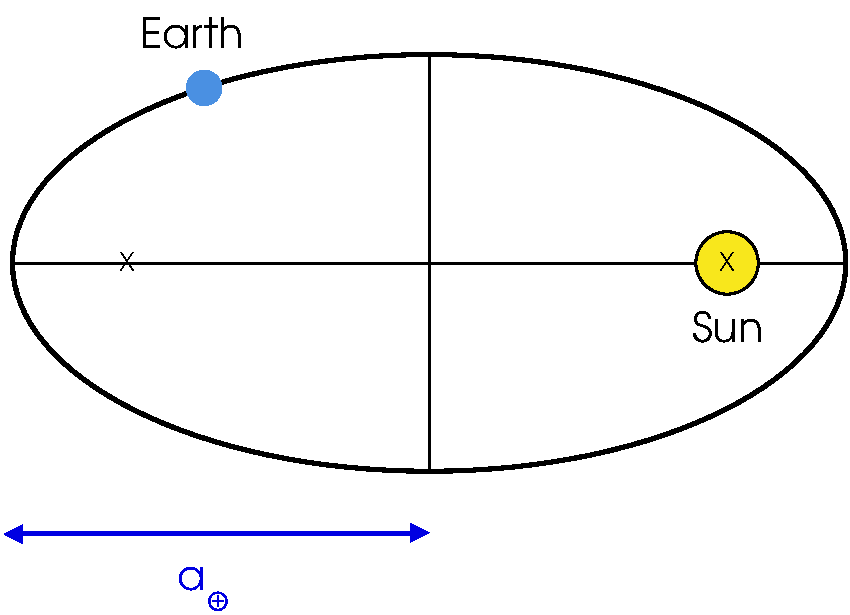
\includegraphics[width=0.60\linewidth]{fig/earth-semi-major-axis}
    \caption{Semi-major axis of Earth's elliptical orbit, used as the characteristic length of the system}
    \label{fig:earth-semi-major-axis}
\end{figure}

Looking at the \(p_j\) from \cref{eq:pr,eq:ptheta,eq:pphi} we can infer their units:

\begin{align}
    k_{pr} &= \frac{k_m}{k_r k_t} \\[0.2cm]
    k_{p\theta} &= \frac{k_m k_r^2}{k_t} = k_{pr} k_r \\[0.2cm]
    k_{p\phi} &= k_{p\theta}
\end{align}

We now introduce the quantity

\begin{equation}
    b_j = \frac{p_j}{m_s}.
\end{equation}
It proves useful to introduce into Hamilton's equations because the mass cancels out (as expected from Newton's 2nd Law, and thus removes the need for introducing  selecting characteristic mass \(k_m\). We will treat the interpretation later. \(b_j\) has units:

\begin{align}
    k_{br} = \frac{k_{pr}}{k_m} = \frac{k_r}{k_t} \\[0.2cm]
    k_{b\theta} = \frac{k_{p\theta}}{k_m} = \frac{k_r^2}{k_t} \\[0.2cm]
    k_{b\phi} = \frac{k_{p\phi}}{k_m} = \frac{k_r^2}{k_t}
\end{align}

For the \(q_j\), \cref{eq:rdot,eq:thetadot,eq:phidot}, we set \(b_j = \frac{p_j}{m_s}\) and nondimensionalize:

\begin{align}
    \od{r}{t} &= \frac{\blue{p_r}}{\blue{p_r}} \\[0.2cm]
    \Leftrightarrow \od{r}{t} &= \blue{b_r} \\[0.2cm]
    \Leftrightarrow \frac{k_r}{k_t} \od{R}{T} &= k_{br} B_R,
\end{align}
so we get
\begin{empheq}[box=\widefbox]{align}
    \label{eq:Rdot}
    \dot{R} = B_R
\end{empheq}

\begin{align}
    \od{\theta}{t} &= \frac{\blue{p_\theta}}{\blue{m_s} r^2} \\[0.2cm]
    \Leftrightarrow \od{\theta}{t} &= \frac{\blue{b_\theta}}{r^2} \\[0.2cm]
    \Leftrightarrow \od{\theta}{t} &= \frac{b_\theta}{r^2} \\[0.2cm]
    \Leftrightarrow \frac{1}{k_t} \od{\theta}{T} &= \frac{k_{b\theta}}{k_r^2} \frac{B_\theta}{R^2},
\end{align}
so we get
\begin{empheq}[box=\widefbox]{align}
    \label{eq:thetadot-nondim}
    \dot{\theta} = \frac{B_\theta}{R^2}
\end{empheq}

\begin{align}
    \od{\phi}{t} &= \frac{\blue{p_\phi}}{{\blue{m_s}} r^2 \sin^2{\theta}} \\[0.3cm]
    \Leftrightarrow \od{\phi}{t} &= \frac{\blue{b_\phi}}{r^2 \sin^2{\theta}}  \\[0.3cm]
    \Leftrightarrow \frac{1}{k_t} \frac{\Phi}{T} &= \frac{k_\phi}{k_r^2} \frac{B_\phi}{R^2 \sin^2{\theta}},
\end{align}
so we get
\begin{empheq}[box=\widefbox]{align}
    \label{eq:phidot-nondim}
    \dot{\phi} = \frac{B_\phi}{R^2 \sin^2{\theta}}
\end{empheq}

For the \(p_j\), \cref{eq:prdot,eq:pthetadot,eq:pphidot} , we first divide by \(m_s\) then set \(b_j = \frac{p_j}{m_s}\) (\blue{relevant terms marked in blue}) and \(\mu_k = G M_k\):

\begin{align}
    \begin{split}
        \od{\blue{p_r}}{t} = -\pd{H}{q_r} &= \frac{\blue{p_\theta^2}}{\blue{m_s} r^3} + \frac{\blue{p_\phi^2}}{\blue{m_s} r^3 \sin^2{\theta} } \\
        &+ G \blue{m_s} \\
        &\sum\limits_{k} M_k \frac{-r + r_k \left(\cos{\theta}\cos{\theta_k} + \sin{\theta}\sin{\theta_k}\cos{(\phi - \phi_k)}\right)}{\left[r^2 + r_k^2 - 2 r r_k \left(\cos{\theta}\cos{\theta_k} + \sin{\theta}\sin{\theta_k}\cos{(\phi - \phi_k)} \right) \right]^{3/2}},
    \end{split} \\[0.3cm]
    \begin{split}
        \Leftrightarrow \od{\blue{b_r}}{t} &= \frac{\blue{b_\theta^2}}{r^3} + \frac{\blue{b_\phi^2}}{r^3 \sin^2{\theta} } \\
        &+ \sum\limits_{k} \mu_k \frac{-r + r_k \left(\cos{\theta}\cos{\theta_k} + \sin{\theta}\sin{\theta_k}\cos{(\phi - \phi_k)}\right)}{\left[r^2 + r_k^2 - 2 r r_k \left(\cos{\theta}\cos{\theta_k} + \sin{\theta}\sin{\theta_k}\cos{(\phi - \phi_k)} \right) \right]^{3/2}}.
    \end{split}
\end{align}
And finally we nondimensionalize:
\begin{align}
    \begin{split}
        \Leftrightarrow \teal{\frac{k_{br}}{k_t}} \od{B_R}{T} &= \orange{\frac{k_{b\theta}^2}{k_r^3}} \frac{B_\theta^2}{R^3} + \orange{\frac{k_{b\phi}^2}{k_r^3}} \frac{B_\phi^2}{R^3 \sin^2{\theta} } \\
        &+ \red{\frac{k_r^3}{k_t^2}\frac{1}{k_r^2}} \\
        & \sum\limits_{k} \eta_k \frac{-R + R_k \left(\cos{\theta}\cos{\theta_k} + \sin{\theta}\sin{\theta_k}\cos{(\phi - \phi_k)}\right)}{\left[R^2 + R_k^2 - 2 R R_k \left(\cos{\theta}\cos{\theta_k} + \sin{\theta}\sin{\theta_k}\cos{(\phi - \phi_k)} \right) \right]^{3/2}},
    \end{split}
\end{align}

where the characteristic units are colored teal, orange and red, \([\mu] = [G] [M_k] = \frac{k_r^3}{k_m k_t^2} k_m = \frac{k_r^3}{k_t^2} \), the first part of the red factor, the second part being from the fraction inside the summation, having units \(\frac{1}{k_r^2}\). Dividing \(\frac{k_{br}}{k_t}\) over from the left-hand side the units cancel as they must:

\begin{align}
    & \teal{\frac{k_t}{k_{br}}} \orange{\frac{k_{b\theta}^2}{k_r^3} } \\
    = &\frac{k_t^2}{k_r} \frac{k_r^4}{k_t^2 k_r^3}\\
    = &1,
\end{align}
and equivalently same for the second orange since \(k_\theta\) and \(k_\phi\) have the same units. And the red terms:

\begin{align}
    & \teal{\frac{k_t}{k_{br}}} \red{\frac{k_r^3}{k_t^2}\frac{1}{k_r^2}} \\
    = &\frac{k_t^2}{k_r} \frac{k_r^3}{k_t^2} \frac{1}{k_r^2} \\
    = &1
\end{align}

and we are left with the nondimensionalized equation:
\begin{empheq}[box=\widefbox]{align}
    \label{eq:Brdot}
    \dot{B}_r = &\frac{B_\theta^2}{R^3} + \frac{B_\phi^2}{R^3 \sin^2{\theta}} \\
    & + \sum\limits_{k} \eta_k \frac{-R + R_k \left(\cos{\theta}\cos{\theta_k} + \sin{\theta}\sin{\theta_k}\cos{(\phi - \phi_k)}\right)}{\left[R^2 + R_k^2 - 2 R R_k \left(\cos{\theta}\cos{\theta_k} + \sin{\theta}\sin{\theta_k}\cos{(\phi - \phi_k)} \right) \right]^{3/2}} \notag
\end{empheq}

The exact same procedure for \(\dot{p_\theta}\) and \(\dot{p}_\phi\) gives us:

\begin{empheq}[box=\widefbox]{align}
    \label{eq:Bthetadot}
    \dot{B}_\theta = &\frac{B_\phi^2}{R^2 \sin^2{\theta} \tan{\theta}} \\
    &+ \sum\limits_{k} \eta_k \frac{R R_k \left[-\sin{\theta}\cos{\theta_k} + \cos{\theta}\sin{\theta_k}\cos{(\phi - \phi_k)} \right]}{\left[R^2 + R_k^2 - 2 R R_k \left(\cos{\theta}\cos{\theta_k} + \sin{\theta}\sin{\theta_k}\cos{(\phi - \phi_k)} \right) \right]^{3/2}} \notag
\end{empheq}

\begin{empheq}[box=\widefbox]{align}
    \label{eq:Bphidot}
    \dot{B}_\phi = &\sum\limits_{k} \eta_k \frac{- R R_k \sin{\theta}\sin{\theta_k}\sin{(\phi - \phi_k)}}{\left[R^2 + R_k^2 - 2 R R_k \left(\cos{\theta}\cos{\theta_k} + \sin{\theta}\sin{\theta_k}\cos{(\phi - \phi_k)} \right) \right]^{3/2}}
\end{empheq}

Finally we can get the nondimensionalize \(H\) by the same method. Again we first divide by \(m_s\) to obtain ``Hamiltonian per spacecraft mass'', \(H/m_s = H_m\):

\begin{equation*}
    \begin{aligned}
        H &= \frac{p_r^2}{2 m_s} + \frac{p_\theta^2}{2 m_s r^2} + \frac{p_\phi^2}{2 m_s r^2 \sin^2{\theta}} \\
        &- G m_s \sum\limits_{k} \frac{M_k}{\sqrt{r^2 + r_k^2 - 2 r r_k \left[\cos{\theta}\cos{\theta_k}+\sin{\theta}\sin{\theta_k}\cos{(\phi - \phi_k})\right]}},
    \end{aligned}
\end{equation*}

\begin{equation}
    \begin{aligned}
        \Leftrightarrow H_m &= \frac{b_r^2}{2} + \frac{b_\theta^2}{2 r^2} + \frac{b_\phi^2}{2 r^2 \sin^2{\theta}} \\
        &- \sum\limits_{k} \mu_k \frac{1}{\sqrt{r^2 + r_k^2 - 2 r r_k \left[\cos{\theta}\cos{\theta_k}+\sin{\theta}\sin{\theta_k}\cos{(\phi - \phi_k})\right]}},
    \end{aligned}
\end{equation}

and then use our characteristic units to get \(\mathcal{H}_m\):

\begin{equation}
    \begin{aligned}
        \Leftrightarrow \mathcal{H}_m &= \frac{B_r^2}{2} + \frac{B_\theta^2}{2 R^2} + \frac{B_\phi^2}{2 R^2 \sin^2{\theta}} \\
        &- \sum\limits_{k} \eta_k \frac{1}{\sqrt{R^2 + R_k^2 - 2 R R_k \left[\cos{\theta}\cos{\theta_k}+\sin{\theta}\sin{\theta_k}\cos{(\phi - \phi_k})\right]}}. \label{eq:HH_m}
    \end{aligned}
\end{equation}

As an overview, \cref{apx:hr4b-overview} shows all six nondimensionalized equations of motion one a single page.

\subsection{H-R4B Numerical Integration Algorithm}

\subsubsection{Symplectic Euler}
In the explicit Euler, all quantities from the Hamiltonian derivative on the right hand refer to the old time step \(0\) ($i$). In the implicit, they are all referring to the new time step \(1\) ($i+1$), which results in implicit equations that can typically only be solved numerically.

The symplectic Euler is mixture between explicit and implicit Euler \cite{Hairer}:

\begin{equation}
    \begin{split} \label{eq:symplectic-euler1}
        \vec{q}_1 = \vec{q}_0 + h \pd{H}{\vec{p}}(q_0, p_1) \\
        \vec{p}_1 = \vec{p}_0 - h \pd{H}{\vec{q}}(q_0, p_1)
    \end{split}
\end{equation}

or

\begin{equation}
    \begin{split} \label{eq:symplectic-euler2}
        \vec{q}_1 = \vec{q}_0 + h \pd{H}{\vec{p}}(q_1, p_0) \\
        \vec{p}_1 = \vec{p}_0 - h \pd{H}{\vec{q}}(q_1, p_0)
    \end{split}
\end{equation}

One can choose whichever is easier to solve for the equations at hand. We choose the latter form \cref{eq:symplectic-euler2} so with our Hamiltonian \cref{eq:HH_m} we get
\begin{align}
    R_1 &= R_0 + h B_{r,0} \label{eq:symplectic-euler-R_1}, \\[0.4cm]
    \theta_1 &= \theta_0 + h \frac{B_{\theta,0}}{R_1^2}, \label{eq:symplectic-euler-theta_1} \\[0.4cm]
    \phi_1 &= \phi_0 + h \frac{B_{\phi,0}}{R_1^2 \sin^2{\theta_1}}, \label{eq:symplectic-euler-phi_1}
\end{align}
\begin{align}    
    \begin{aligned}
        B_{r,1} = & B_{r,0} + h \left[ \frac{B_{\theta,0}^2}{R_1^3} + \frac{B_{\phi,0}^2}{R_1^3 \sin^2{\theta_1}} \right. \\
        & \hspace{-21.0pt} + \left. \sum\limits_{k} \eta_k \frac{-R_1 + R_{k,1} \left(\cos{\theta_1}\cos{\theta_{k,1}} + \sin{\theta_1}\sin{\theta_{k,1}}\cos{(\phi_1 - \phi_{k,1})}\right)}{\left[R_1^2 + R_{k,1}^2 -2 R_1 R_{k,1}^2 \left(\cos{\theta_1}\cos{\theta_{k,1}} + \sin{\theta_1}\sin{\theta_{k,1}}\cos{(\phi_1 - \phi_{k,1})} \right) \right]^{3/2}} \right] , \label{eq:symplectic-euler-Br_1}
    \end{aligned} \\[0.4cm]
    \begin{aligned}
        B_{\theta,1} = & B_{\theta,0} + h \left[ \frac{B_{\phi,0}^2}{R_1^2 \sin^2{\theta_1} \tan{\theta_1}} \right. \\
        & \hspace{-21.0pt} + \left. \sum\limits_{k} \eta_k \frac{R_1 R_{k,1} \left[-\sin{\theta_1}\cos{\theta_{k,1}} + \cos{\theta_1}\sin{\theta_{k,1}}\cos{(\phi_1 - \phi_{k,1})} \right]}{\left[R_1^2 + R_{k,1}^2 -2 R_1 R_{k,1}^2 \left(\cos{\theta_1}\cos{\theta_{k,1}} + \sin{\theta_1}\sin{\theta_{k,1}}\cos{(\phi_1 - \phi_{k,1})} \right) \right]^{3/2}} \right], \label{eq:symplectic-euler-Btheta_1}
    \end{aligned} \\[0.4cm]
    \begin{aligned}
        B_{\phi,1} = & B_{\phi,0} + h \left[ \vphantom{\frac12} \right.\\
        & \hspace{-21.0pt} \hphantom{+} \left. \sum\limits_{k} \eta_k \frac{- R_1 R_{k,1} \sin{\theta_1}\sin{\theta_{k,1}}\sin{(\phi_1 - \phi_{k,1})}}{\left[R_1^2 + R_{k,1}^2 -2 R_1 R_{k,1}^2 \left(\cos{\theta_1}\cos{\theta_{k,1}} + \sin{\theta_1}\sin{\theta_{k,1}}\cos{(\phi_1 - \phi_{k,1})} \right) \right]^{3/2}} \right]. \label{eq:symplectic-euler-Bphi_1}
    \end{aligned}
\end{align}
As we can see, we are lucky with this Hamiltonian since we can simply run all steps in the order above, \cref{eq:symplectic-euler-R_1,eq:symplectic-euler-theta_1,eq:symplectic-euler-phi_1,eq:symplectic-euler-Br_1,eq:symplectic-euler-Btheta_1,eq:symplectic-euler-Bphi_1} without needing to solve any implicit equations.

\section{Interplanetary Transfer Orbits}

\subsection{The Challenges of a Mars Transfer Orbit}
Making the trip to Mars from Earth is not a simple task. 

\subsection{Transfer Orbit to Mars: 2D Patched Conic Approximation} \label{sec:2d-patched-conic}
For now we want to do away with many of the complexities described in the previous section, and make an approximation, which will give us a sense of the key numbers of getting to Mars:
\begin{enumerate}
	\item Delta-v for Mars Orbit Insertion (MOI) at Earth.
	\item Delta-v for arrival into circular orbit at Mars.
	\item Relative positions of Earth and Mars for optimal Hohmann trajectory.
	\item Travel time for optimal Hohmann trajectory.
\end{enumerate}

Knowing this we have a first good guess on initial conditions to put into the interplanetary 3D simulator, for which we can search for optimal parameters nearby for some good low-delta-v trajectories to mars. To approximate these numbers we can use the \emph{patched conic approximation}.

First we recall that there are four possible orbit types in a two-body system that are all conic sections: circular, elliptic, parabolic and hyperbolic (and the circular is actually a special case of the elliptic), see \cref{fig:conics-and-orbits}.

\begin{figure}[ht]
    \centering
    \subfloat[Conic sections. The parabola is created from an intersecting plane parallel to the cone (Image: \cite{MagisterMathematicae} (modified)).]{
        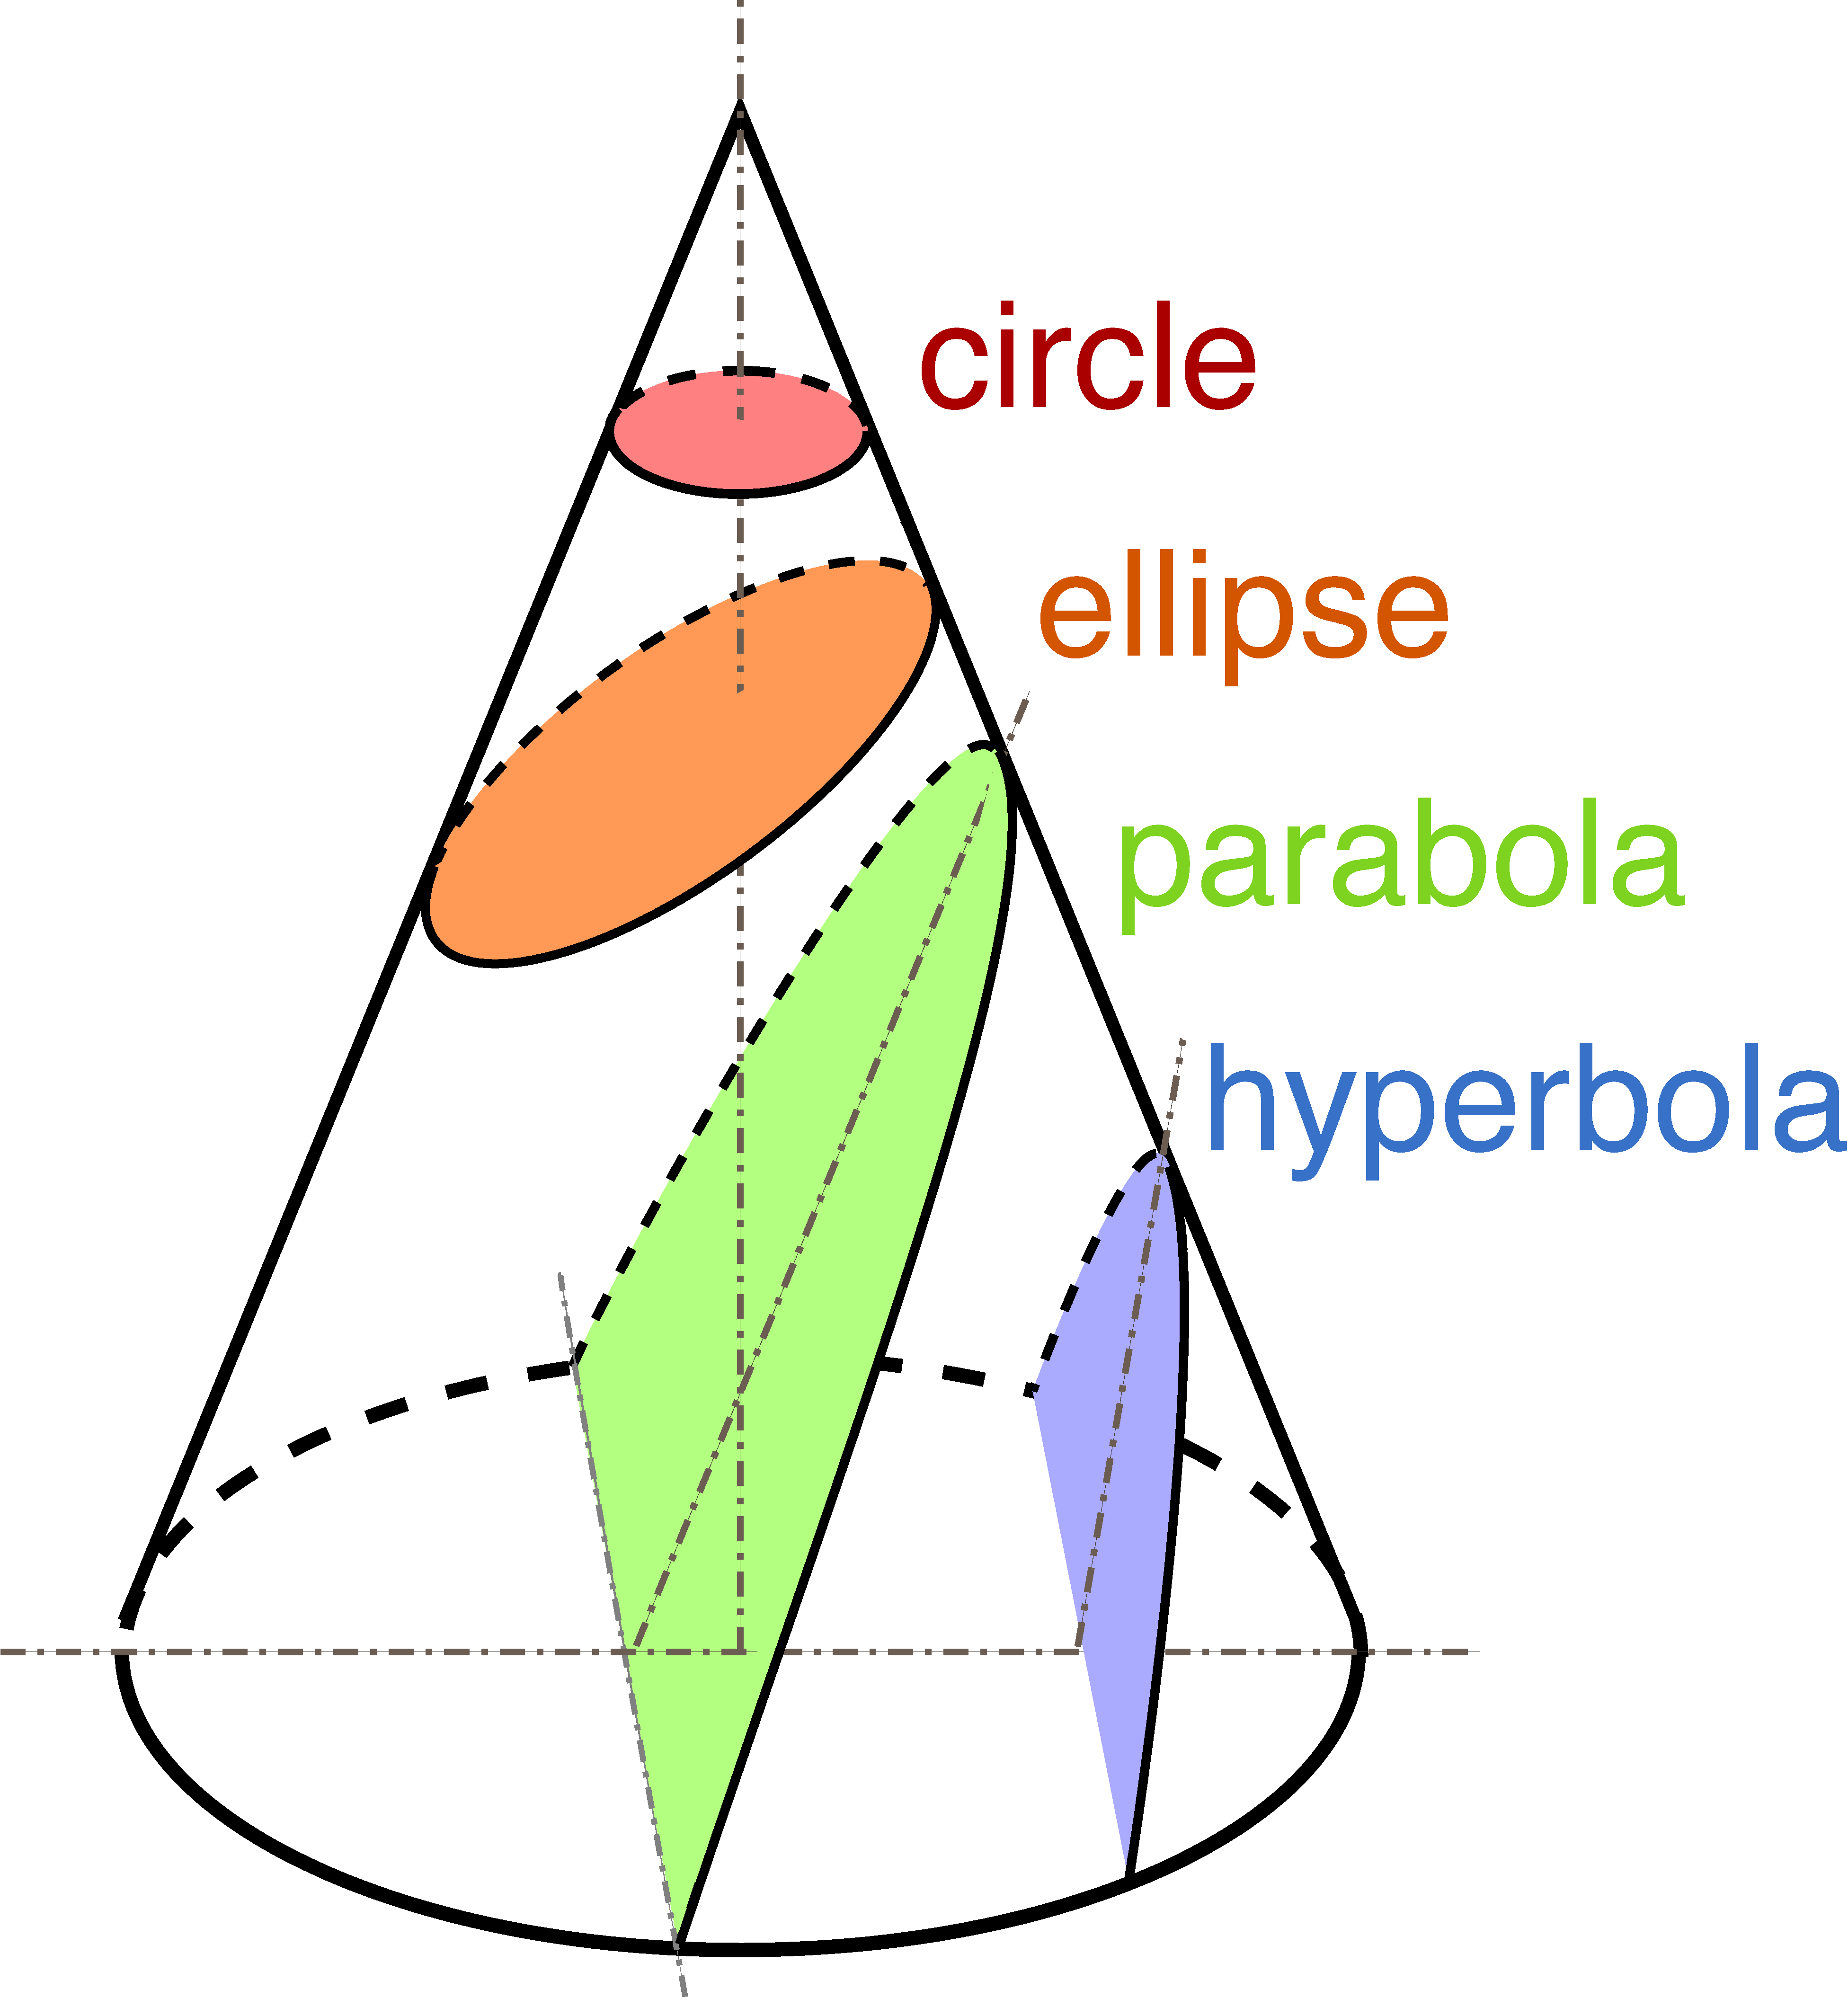
\includegraphics[width=0.47\linewidth]{fig/Conic_Sections2.pdf}
        \label{fig:conic-sections}
    }
    \hfill
    \subfloat[Examples of the four orbit types of a two-body system and their eccentricities (Image: \cite{Seahen} (modified)).]{
        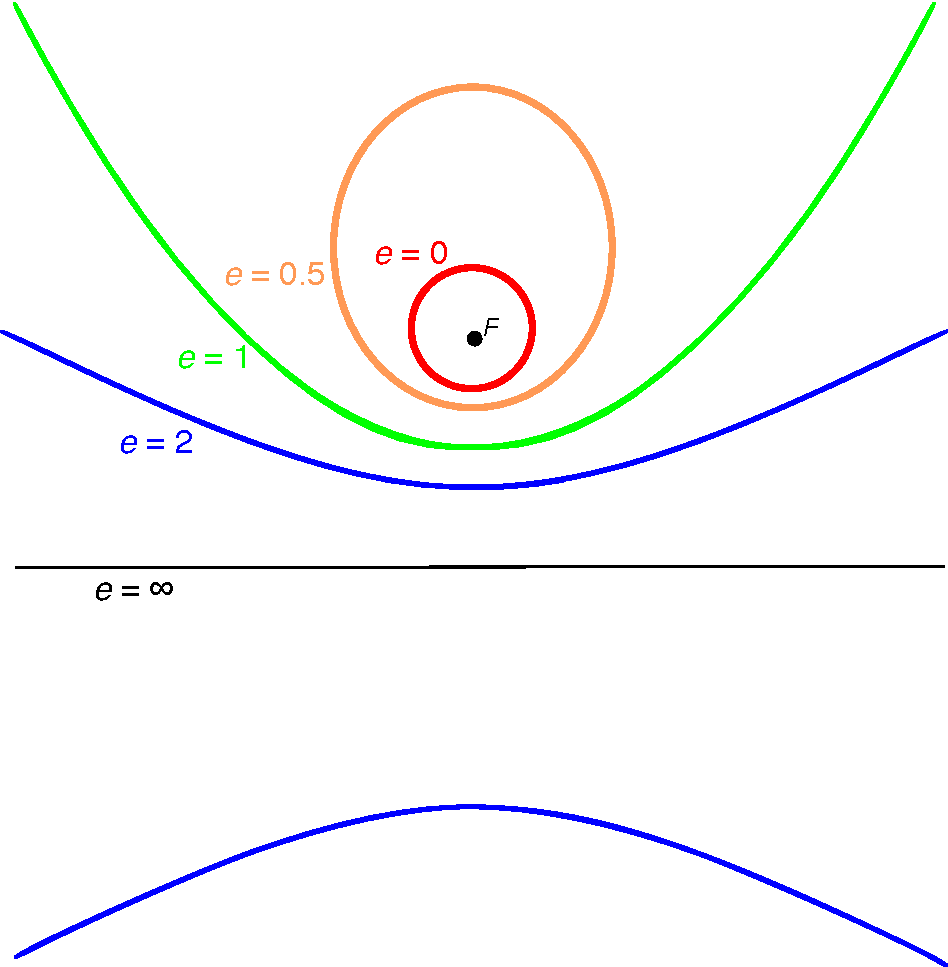
\includegraphics[width=0.47\linewidth]{fig/Eccentricity.pdf}
        \label{fig:orbit-types}
    }
    \caption{The four types of conic sections, corresponding to the four kinds of orbits for a two-body gravitational system. Some authors count three types, with the circle being a special case of the ellipse.}
    \label{fig:conics-and-orbits}
\end{figure}

These four orbit types are characterized by the orbit specific energy (mechanical energy per mass) or equivalently by the ranges of eccentricity, see table in \cref{tab:orbit-type-properties}. As the table shows, a negative mechanical energy corresponds to a closed orbit (either circular or elliptical), zero energy corresponds to a parabolic orbit, i.e. an escape velocity orbit that occurs when a satellite is moving with \emph{just} enough speed with respect to a central body that it's speed goes towards zero at infinity. Finally, positive mechanical energy gives hyperbolic orbits.

\begin{table}[tbp]
    \centering
    \begin{tabular}{@{}llll@{}}
    \toprule
    Conic Section & Eccentricity    & Semi-major axis & Energy  \\ \midrule
    Circle        & $0$             & = radius        & $<0$    \\
    Ellipse       & $0 < e < 1$     & $>0$            & $<0$    \\
    Parabola      & 1               & infinity        & $0$     \\
    Hyperbola     & $>1$            & $<0$            & $>0$    \\ \bottomrule
    \end{tabular}
    \caption{Properties of the four orbit types, characterized by their specific energy and eccentricity \cite{Braeunig}.}
    \label{tab:orbit-type-properties}
\end{table}


For a interplanetary transfer orbit we can use the Hohmann transfer orbit as the ``base transfer orbit'' and make some modifications. We recall that the Hohmann transfer is an elliptical orbit that brings a satellite between two different circular orbits around a central body by applying an instantaneous burn twice as depicted in \cref{fig:hohmann}.

\begin{figure}[ht]
    \centering
    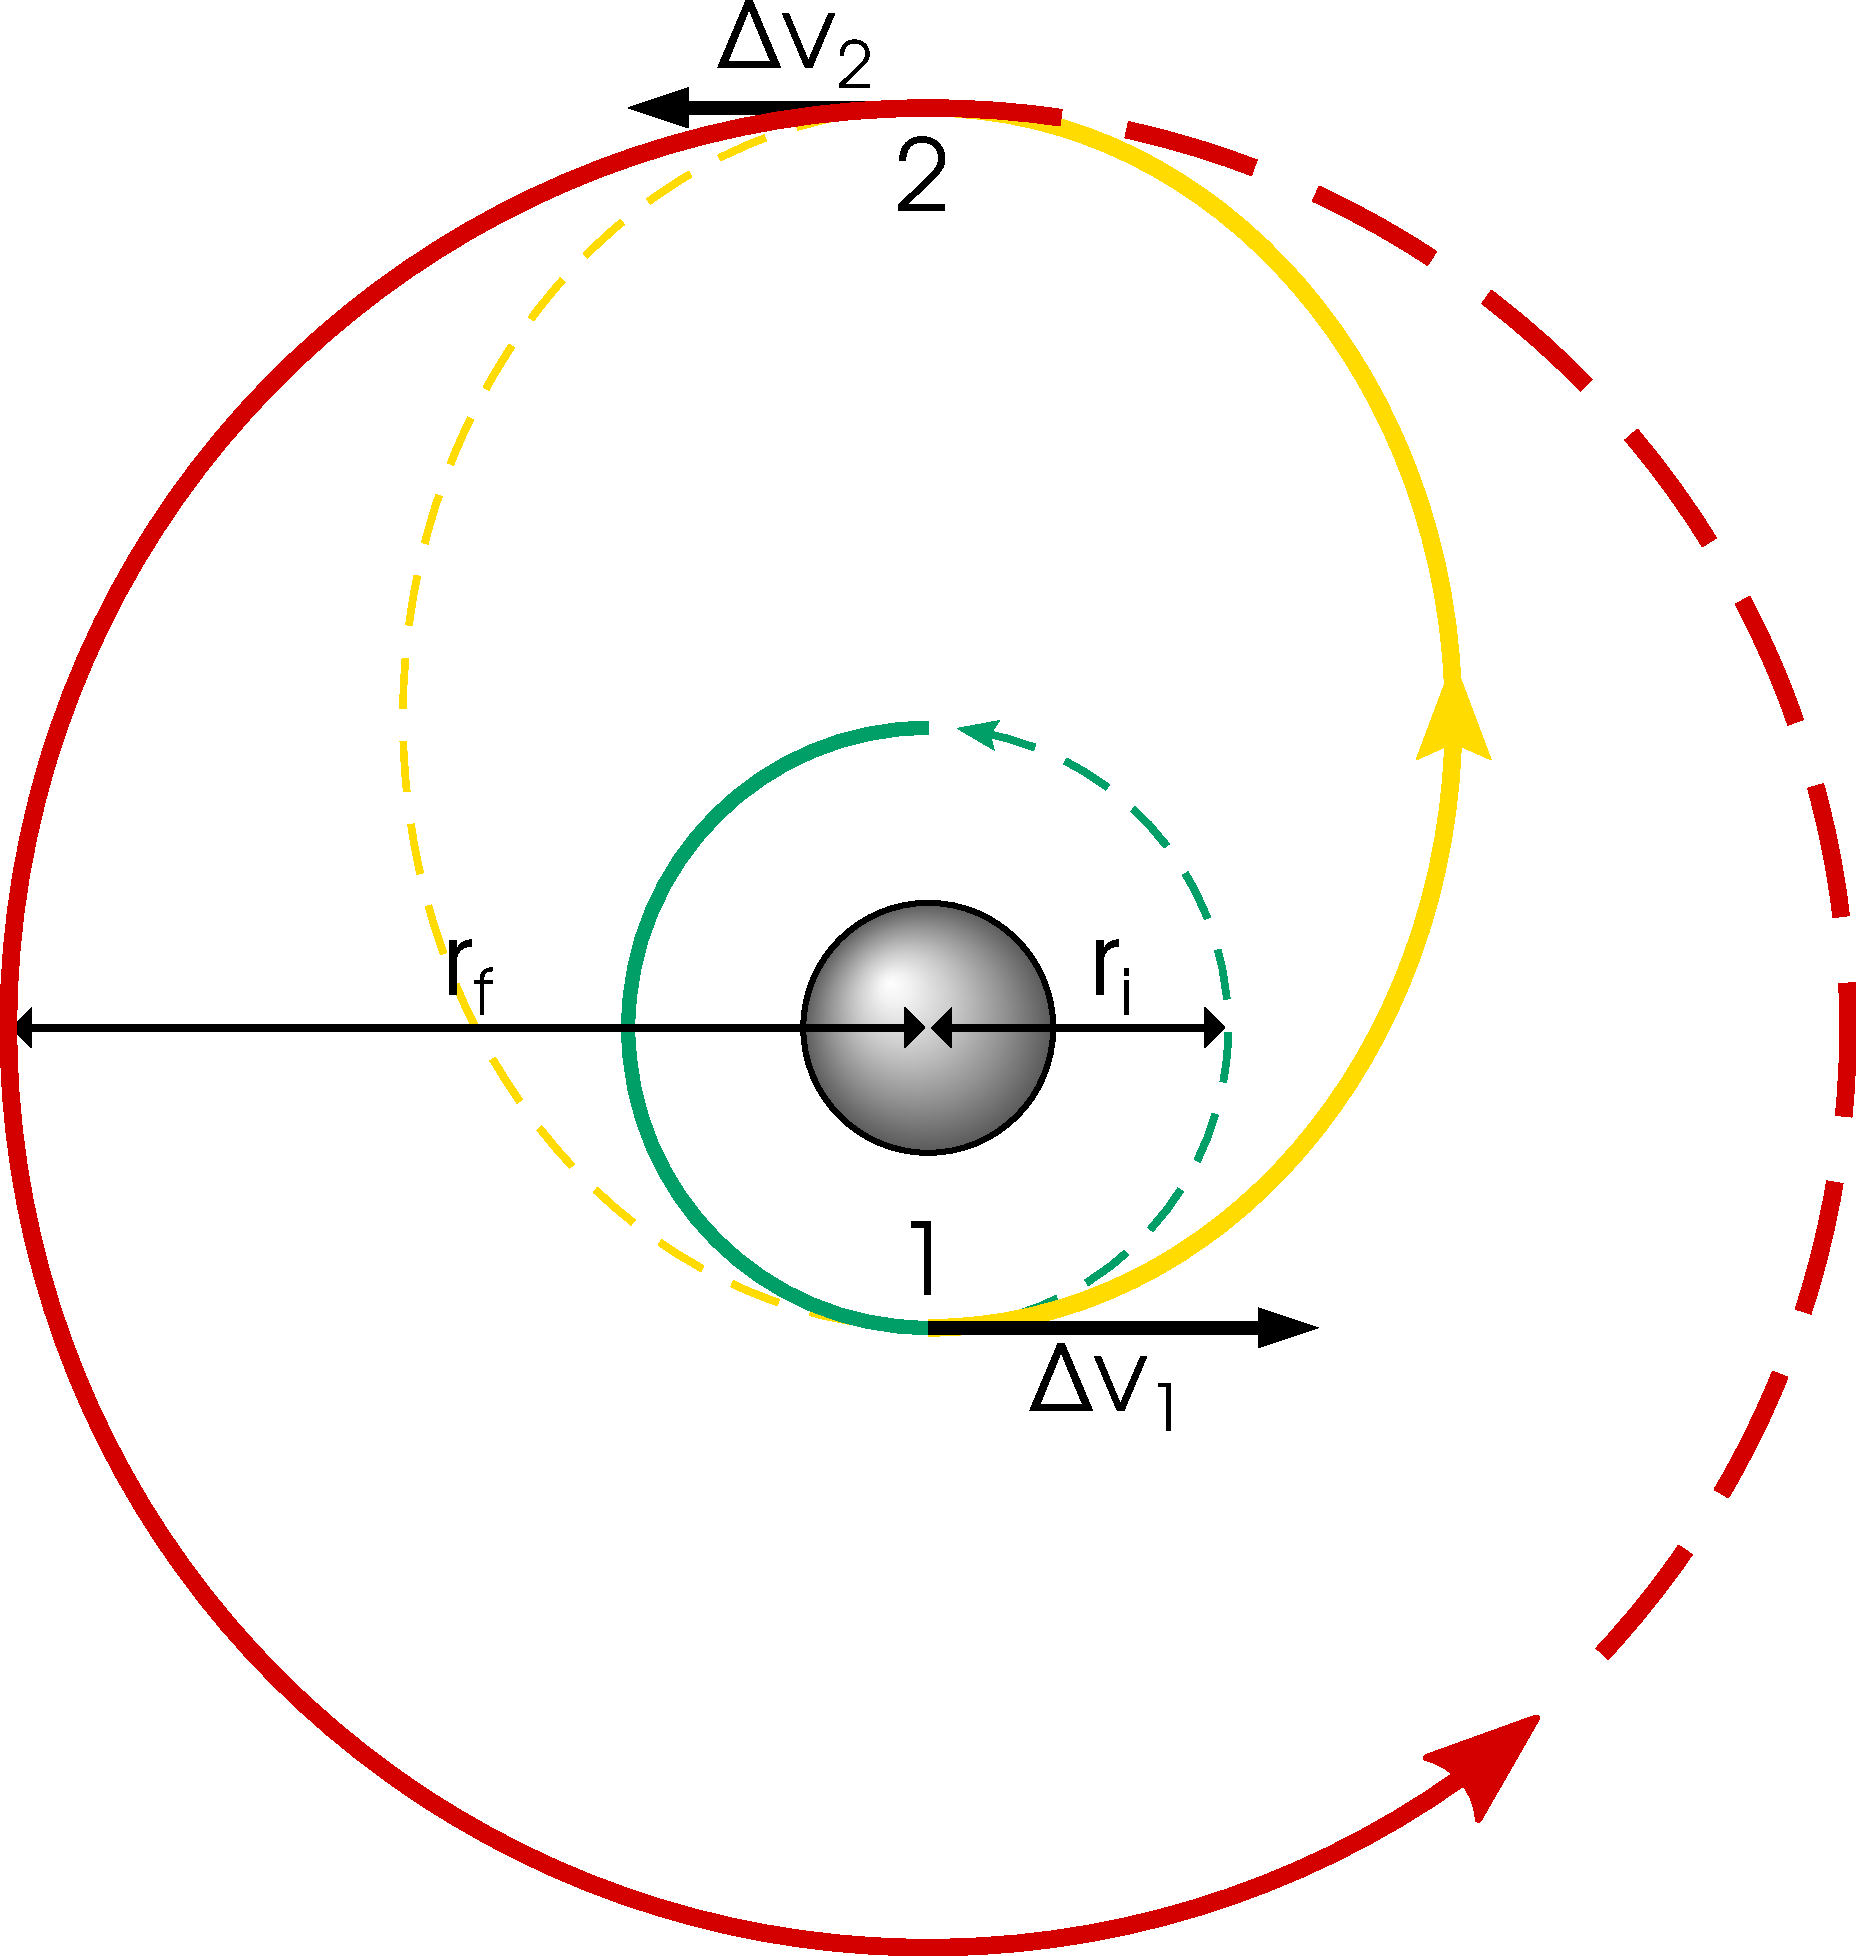
\includegraphics[width=0.4\linewidth]{fig/hohmann.pdf}
    \caption{Hohmann Transfer orbit that brings the satellite from one circular orbit around a central body to another circular orbit via two burns (Image: \cite{Leafnode} (modified)).}
    \label{fig:hohmann}
    \end{figure}

This approximation assumes only one central body. However in our system, we have three central bodies of interest: Earth, Sun and Mars. Each is the dominant body at various points of the journey. We start in a circular orbit around Earth, burn into an elliptical orbit around the Sun and arrive to Mars, burning to a circular orbit again. We can model the transfer orbit to Mars by patching three conic sections:

\begin{enumerate}
	\item Hyperbolic departure orbit (Geocentric reference frame).
	\item Elliptical transfer orbit (Heliocentric reference frame).
	\item Hyperbolic arrival orbit (Mars-centric reference frame).
\end{enumerate}

\cref{fig:Hohmann-to-mars-heliocentric} show necessary speeds on Hohmann orbit and the orbit speed of Earth and Mars. 

\begin{figure}[ht]
    \centering
    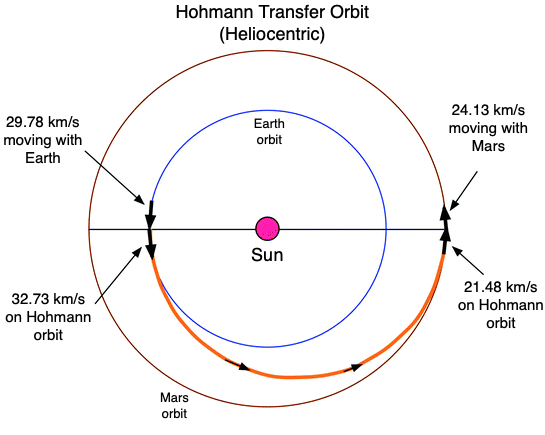
\includegraphics[width=0.7\linewidth]{fig/Hohmann-to-mars-heliocentric.png}
    \caption{Hohmann transfer to Mars with necessary departure speed (periapsis at Earth) and arrival speed (apoapsis at Mars) on Hohmann orbit relative to Sun (Image: \cite[p.~127]{Rapp2016} (modified)).}
    \label{fig:Hohmann-to-mars-heliocentric}
\end{figure}


Why are the departure and arrival orbits modelled as hyperbolic? It turns out that we need extra speed from LEO to enter a transfer orbit that intersects Mars, meaning we need some velocity in excess to escape velocity. Likewise we \emph{always} arrive at other bodies in a hyperbolic orbit as seen from that body. If we started with zero speed approaching from infinitely far away and waited a duration approaching infinity, we would get the escape velocity when reaching the planet (this is just escaping with the exact escape velocity in reverse). But since we in practice always come with some other speed than the body we approach (here Mars), get arrive with speed in excess to the escape velocity, hence along a hyperbolic orbit, as shown in table in \cref{tab:orbit-type-properties}.

As \cref{fig:Hohmann-to-mars-heliocentric} shows, we arrive at Mars' orbit with less speed than Mars \emph{if Mars wasn't there}, but actually need to slow down due to the attraction of Mars that results in higher speed to necessary for a circular orbit in target altitude \SI{125}{\km}. Thus overall we get a hyperbolic departure orbit, patched with an elliptical orbit, patched with another hyperbolic arrival orbit, with required speeds as illustrated in figure \cref{fig:Hohmann-to-mars-geocentric-areocentric}.

\begin{figure}[ht]
    \centering
    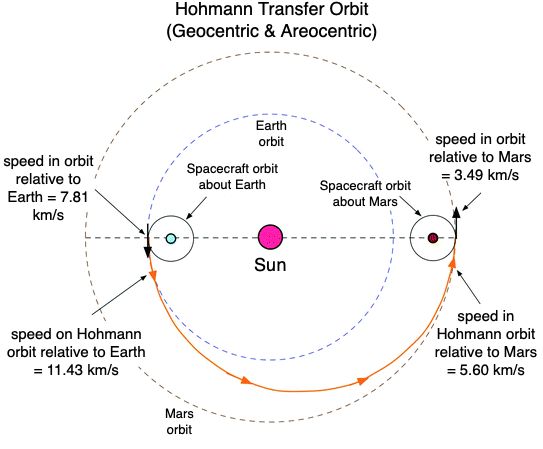
\includegraphics[width=0.7\linewidth]{fig/Hohmann-to-mars-geocentric-areocentric.png}
    \caption{Hohmann transfer to Mars with necessary departure, arrival and parking speeds relative to Earth on the left and Mars on the right (Image: \cite[p.~133]{Rapp2016} (modified)).}
    \label{fig:Hohmann-to-mars-geocentric-areocentric}
\end{figure}

All the numbers of \cref{fig:Hohmann-to-mars-heliocentric,fig:Hohmann-to-mars-geocentric-areocentric} are derived in \cref{apx:mars-hohmann-derivations}, answering our four questions from the beginning of the chapter:

\begin{enumerate}
	\item \SI{3.62}{\km\per\s} needed to depart Earth circular orbit at altitude 160 km on Mars Orbit Insertion (MOI).
	\item \SI{-2.11}{\km\per\s} needed at Mars arrival for circular orbit at \SI{125}{\km} altitude. Just for illustration, we could also apply less burn at Mars at the expense of entering a highly elliptical orbit as \cref{fig:mars-arrival-orbit} shows.
	\item Mars must be $44^\degree$ behind Earth at MOI in order for Mars to be at Hohmann orbit apoapsis at the same time, see \cref{fig:Hohmann-angle}. This happens every 1.6 years \cite{Odenwald} (assuming Earth and Mars and in the same plane and orbit eccentricities are zero).
	\item Travel time for optimal Hohmann trajectory is around 260 days, or around 8.5 months.
\end{enumerate}

These numbers are an important approximate reference point to have when attempting to find low energy transfer orbits to Mars.

\begin{figure}[ht]
    \centering
    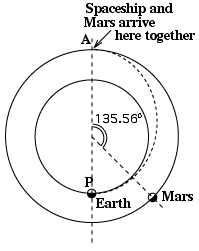
\includegraphics[width=0.35\linewidth]{fig/Hohmann-angle.png}
    \caption{The angle that Mars travels during the Mars Hohmann transfer orbit can easily be calculated as roughly \(136^\degree\), meaning the optimal launch is when Mars is \(44^\degree\) behind Earth in orbit (Image: \cite{Stern}).}
    \label{fig:Hohmann-angle}
\end{figure}

\begin{figure}[ht]
    \centering
    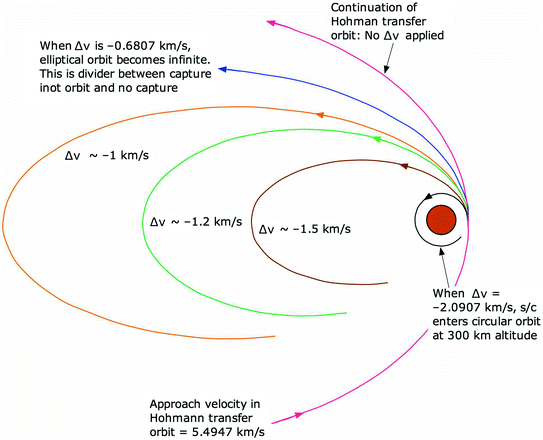
\includegraphics[width=0.85\linewidth]{fig/mars-arrival-orbit.png}
    \caption{Various closed orbits upon arrival depending on applied $\Delta v$ (Image: \cite[p.~137]{Rapp2016} (modified)).}
    \label{fig:mars-arrival-orbit}
\end{figure}

\clearpage

\subsection{Actual Hohmann Transfer Orbit in 3D}
In the previous section we detailed the important patched conic sections model in 2D. In our 3D simulator we will attempt something similar, but take the inclination of Mars' orbital plane into account.

Mars orbital inclination is $1.85^\degree$ to the ecliptic plane. Therefore if one naively tried to rendezvous with Mars in the ecliptic plane it would be \( 1.52\ \text{AU} \cdot 1.85^\degree \pi / 180 = \SI{7.4e6}{\km} \) away. Instead we will attempt a 3D Hohmann transfer orbit as illustrated in \cref{fig:hohmann-transfer-orbit-3D} using the same launch parameters as was found in the 2D hohmann model in \cref{sec:2d-patched-conic}, but allowing the \(\phi\) angle to vary a bit to get slightly out of the plane.

\begin{figure}[ht]
    \centering
    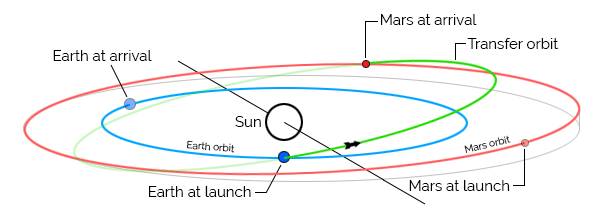
\includegraphics[width=0.90\linewidth]{fig/hohmann-transfer-orbit-3D.png}
    \caption{Hohmann orbit in a 3D model needs a small $\Delta v$ in the $\phi$ direction to get out of the plane in such a way that it will be in the orbital plane at Mars at apoapsis (Image: \cite{Daedalis.de})}
    \label{fig:hohmann-transfer-orbit-3D}
\end{figure}
 